\documentclass[a4paper,12pt]{article}

\usepackage{a4wide}
\usepackage{amsfonts}
\usepackage{amsmath}
\usepackage{amssymb}
\usepackage{lipsum}
\usepackage{hyperref}
\usepackage{cleveref}

\usepackage{graphicx}  % For including images

\usepackage{xcolor}  % For a colorfull presentation
\usepackage{listings}  % For presenting code

\usepackage{float}
\usepackage{hyperref}

% Definition of a style for code, matter of taste
\lstdefinestyle{mystyle}{
  language=Python,
  basicstyle=\ttfamily\footnotesize,
  backgroundcolor=\color[HTML]{F7F7F7},
  rulecolor=\color[HTML]{EEEEEE},
  identifierstyle=\color[HTML]{24292E},
  emphstyle=\color[HTML]{005CC5},
  keywordstyle=\color[HTML]{D73A49},
  commentstyle=\color[HTML]{6A737D},
  stringstyle=\color[HTML]{032F62},
  emph={@property,self,range,True,False},
  morekeywords={super,with,as,lambda},
  literate=%
    {+}{{{\color[HTML]{D73A49}+}}}1
    {-}{{{\color[HTML]{D73A49}-}}}1
    {*}{{{\color[HTML]{D73A49}*}}}1
    {/}{{{\color[HTML]{D73A49}/}}}1
    {=}{{{\color[HTML]{D73A49}=}}}1
    {/=}{{{\color[HTML]{D73A49}=}}}1,
  breakatwhitespace=false,
  breaklines=true,
  captionpos=b,
  keepspaces=true,
  numbers=none,
  showspaces=false,
  showstringspaces=false,
  showtabs=false,
  tabsize=4,
  frame=single,
}
\lstset{style=mystyle}

\begin{document}
\title{Machine Learning A (2026)\\Home Assignment 2}
\author{\color{red}Ludovico Maria Spitaleri, DMH249}
\date{}
\maketitle

% Please leave the table of contents as is, for the ease of navigation for TAs
\tableofcontents % Generates the table of contents
\newpage % Start a new page after the table of contents

% % Placeholder figure
% \begin{figure}[htbp]
%     \centering
%     \includegraphics[width=0.5\linewidth]{example-image}
%     \caption{\lipsum[1][1-3]} % Dummy caption generated using lipsum
%     \label{fig:placeholder}
% \end{figure}



% % Placeholder code
% \begin{lstlisting}
% # Example code
% # Creating an example array
% data = np.array([5, 2, 8, 1, 6])

% # Calculating cumulative sum using cumsum
% cumulative_sum = np.cumsum(data)
% \end{lstlisting}

\section{Preprocessing (35 points)}

\subsection{Importance of Preprocessing (8 points)}

The nearest neighbor to C is B, so BoL should not give hime credit according to
the algorithm.

$$
\begin{aligned}
A: & \sqrt{(21-47)^2 + (36-35)^2} & \approx 26.02 \\
B: & \sqrt{(21-22)^2 + (36-40)^2} & \approx 4.12
\end{aligned}
$$

If instead the income is measured in dollars, A would be the nearest
neighbor, so BoL should give C credit.

$$
\begin{aligned}
A: & \sqrt{(21-47)^2 + (36000 - 35000)^2} & \approx 1000.34 \\
B: & \sqrt{(21-22)^2 + (36000 - 40000)^2} & \approx 4000.00
\end{aligned}
$$

This is because Eucledian distance is not scale-invariant.

\subsection{Input Centering (9 points)}

\subsubsection{(a)}

$$
\begin{aligned}
z_n = x_n - \bar{x} & \implies Z = X - \mathbf{1}\bar{x}^\top \\
& = X - \mathbf{1} \left( \frac{1}{N}X^\top \mathbf{1} \right)^\top \\
& = X - \frac{1}{N}\mathbf{1}\mathbf{1}^\top X \\
& = \left(I - \frac{1}{N}\mathbf{1}\mathbf{1}^\top\right)X \\
& = \gamma X
\end{aligned}
$$

\subsubsection{(b)}

\subsection{Input Whitening (18 points)}

\subsubsection{(a)}

$$
\begin{aligned}
Var(x_1) & = Var(\hat{x}_1) = 1 \\
Var(x_2) & = Var(\sqrt{1-\epsilon^2}\hat{x}_1 + \epsilon \hat{x}_2) \\
    & = (1-\epsilon^2) Var(\hat{x}_1) + \epsilon^2 Var(\hat{x}_2) \\
    & = (1-\epsilon^2)(1) + \epsilon^2(1) \\
    & = 1 \\
Cov(x_1, x_2) & = Cov(\hat{x}_1, \sqrt{1-\epsilon^2}\hat{x}_1 + \epsilon \hat{x}_2) \\
    & = \sqrt{1-\epsilon^2}Cov(\hat{x}_1, \hat{x}_1) + \epsilon Cov(\hat{x}_1, \hat{x}_2) \\
    & = \sqrt{1-\epsilon^2}(1) + 0 \\
    & = \sqrt{1-\epsilon^2}
\end{aligned}
$$

\subsubsection{(b)}
\label{sssec:input-whitening-b}

$$
\begin{aligned}
\hat{x}_1 = x_1, \, \hat{x}_2 = \frac{x_2 - \sqrt{1-\epsilon^2}x_1}{\epsilon} \implies
f(x) & = \hat{w}_1(x_1) + \hat{w}_2\left(\frac{x_2 - \sqrt{1-\epsilon^2}x_1}{\epsilon}\right) \\
    & = \left(\hat{w}_1 - \hat{w}_2\frac{\sqrt{1-\epsilon^2}}{\epsilon}\right)x_1 + \left(\frac{\hat{w}_2}{\epsilon}\right)x_2 \\
    \implies w_1 = \hat{w}_1 - \hat{w}_2\frac{\sqrt{1-\epsilon^2}}{\epsilon} \,, \quad w_2 = \frac{\hat{w}_2}{\epsilon}
\end{aligned}
$$

\subsubsection{(c)}

$$
f(\hat{x}) = \hat{x}_1 + \hat{x}_2 \implies \hat{w}_1 = 1, \, \hat{w}_2 = 1
$$

Plugging these into our equations from \cref{sssec:input-whitening-b}:

$$
w_1 = 1 - \frac{\sqrt{1-\epsilon^2}}{\epsilon}, \quad w_2 = \frac{1}{\epsilon}
$$

The minimum $C$ needed for the constraint $w_1^2 + w_2^2 \le C$ is exactly $w_1^2 + w_2^2$:

$$
\begin{aligned}
C_{min} & = \left(1 - \frac{\sqrt{1-\epsilon^2}}{\epsilon}\right)^2 + \left(\frac{1}{\epsilon}\right)^2 \\
    & = 1 - 2\frac{\sqrt{1-\epsilon^2}}{\epsilon} + \frac{1-\epsilon^2}{\epsilon^2} + \frac{1}{\epsilon^2} \\
    & = 1 - 2\frac{\sqrt{1-\epsilon^2}}{\epsilon} + \frac{2-\epsilon^2}{\epsilon^2} \\
    & = 1 - 2\frac{\sqrt{1-\epsilon^2}}{\epsilon} + \frac{2}{\epsilon^2} - 1 \\
    & = \frac{2}{\epsilon^2} - \frac{2\sqrt{1-\epsilon^2}}{\epsilon}
\end{aligned}
$$

\subsubsection{(d)}

As $\epsilon \to 0$, the dominant term $\frac{2}{\epsilon^2}$ prevails and $C_{min} \to \infty$.
This means that as inputs become highly correlated, the weights required to construct
the target function become infinitely large.

\section{Hoeffding's Bound (15 points)}

$$
\begin{aligned}
\mathbb{E}[X] & = \frac{-2 + 0.8 + 1}{3} = \frac{-0.2}{3} = -\frac{1}{15} \\
\mathbb{E}[S] & = N\mathbb{E}[X] = -\frac{100}{15} = -\frac{20}{3} \\
X \in [a, b] & \text{ with } a = -2, b = 1 \\
\mathbb{P}(S > 22) & \implies \mathbb{P}(S - \mathbb{E}[S] > 22 - \mathbb{E}[S]) \\ \\
& = \mathbb{P}\left(S - \mathbb{E}[S] > \frac{86}{3}\right)
\end{aligned}
$$

Using Hoeffding's Inequality for sums:

$$
\mathbb{P}\left(S - \mathbb{E}[S] \ge \frac{86}{3}\right)
\le \exp\left(-\frac{2 \cdot (\frac{86}{3})^2}{100 \cdot 3^2}\right)
\approx 0.1610
$$

\newpage

\section{Illustration of Markov's, Chebyshev's, and Hoeffding's Inequalities (25 points)}

\paragraph{3.a}

\paragraph{1.}

\begin{lstlisting}
alphas = np.arange(0.5, 1 + 0.05, 0.05) # add step to endpoint to be inclusive
empirical_freq = np.array([np.mean(sample_means >= a) for a in alphas])
\end{lstlisting}

\begin{figure}[H]
    \centering
    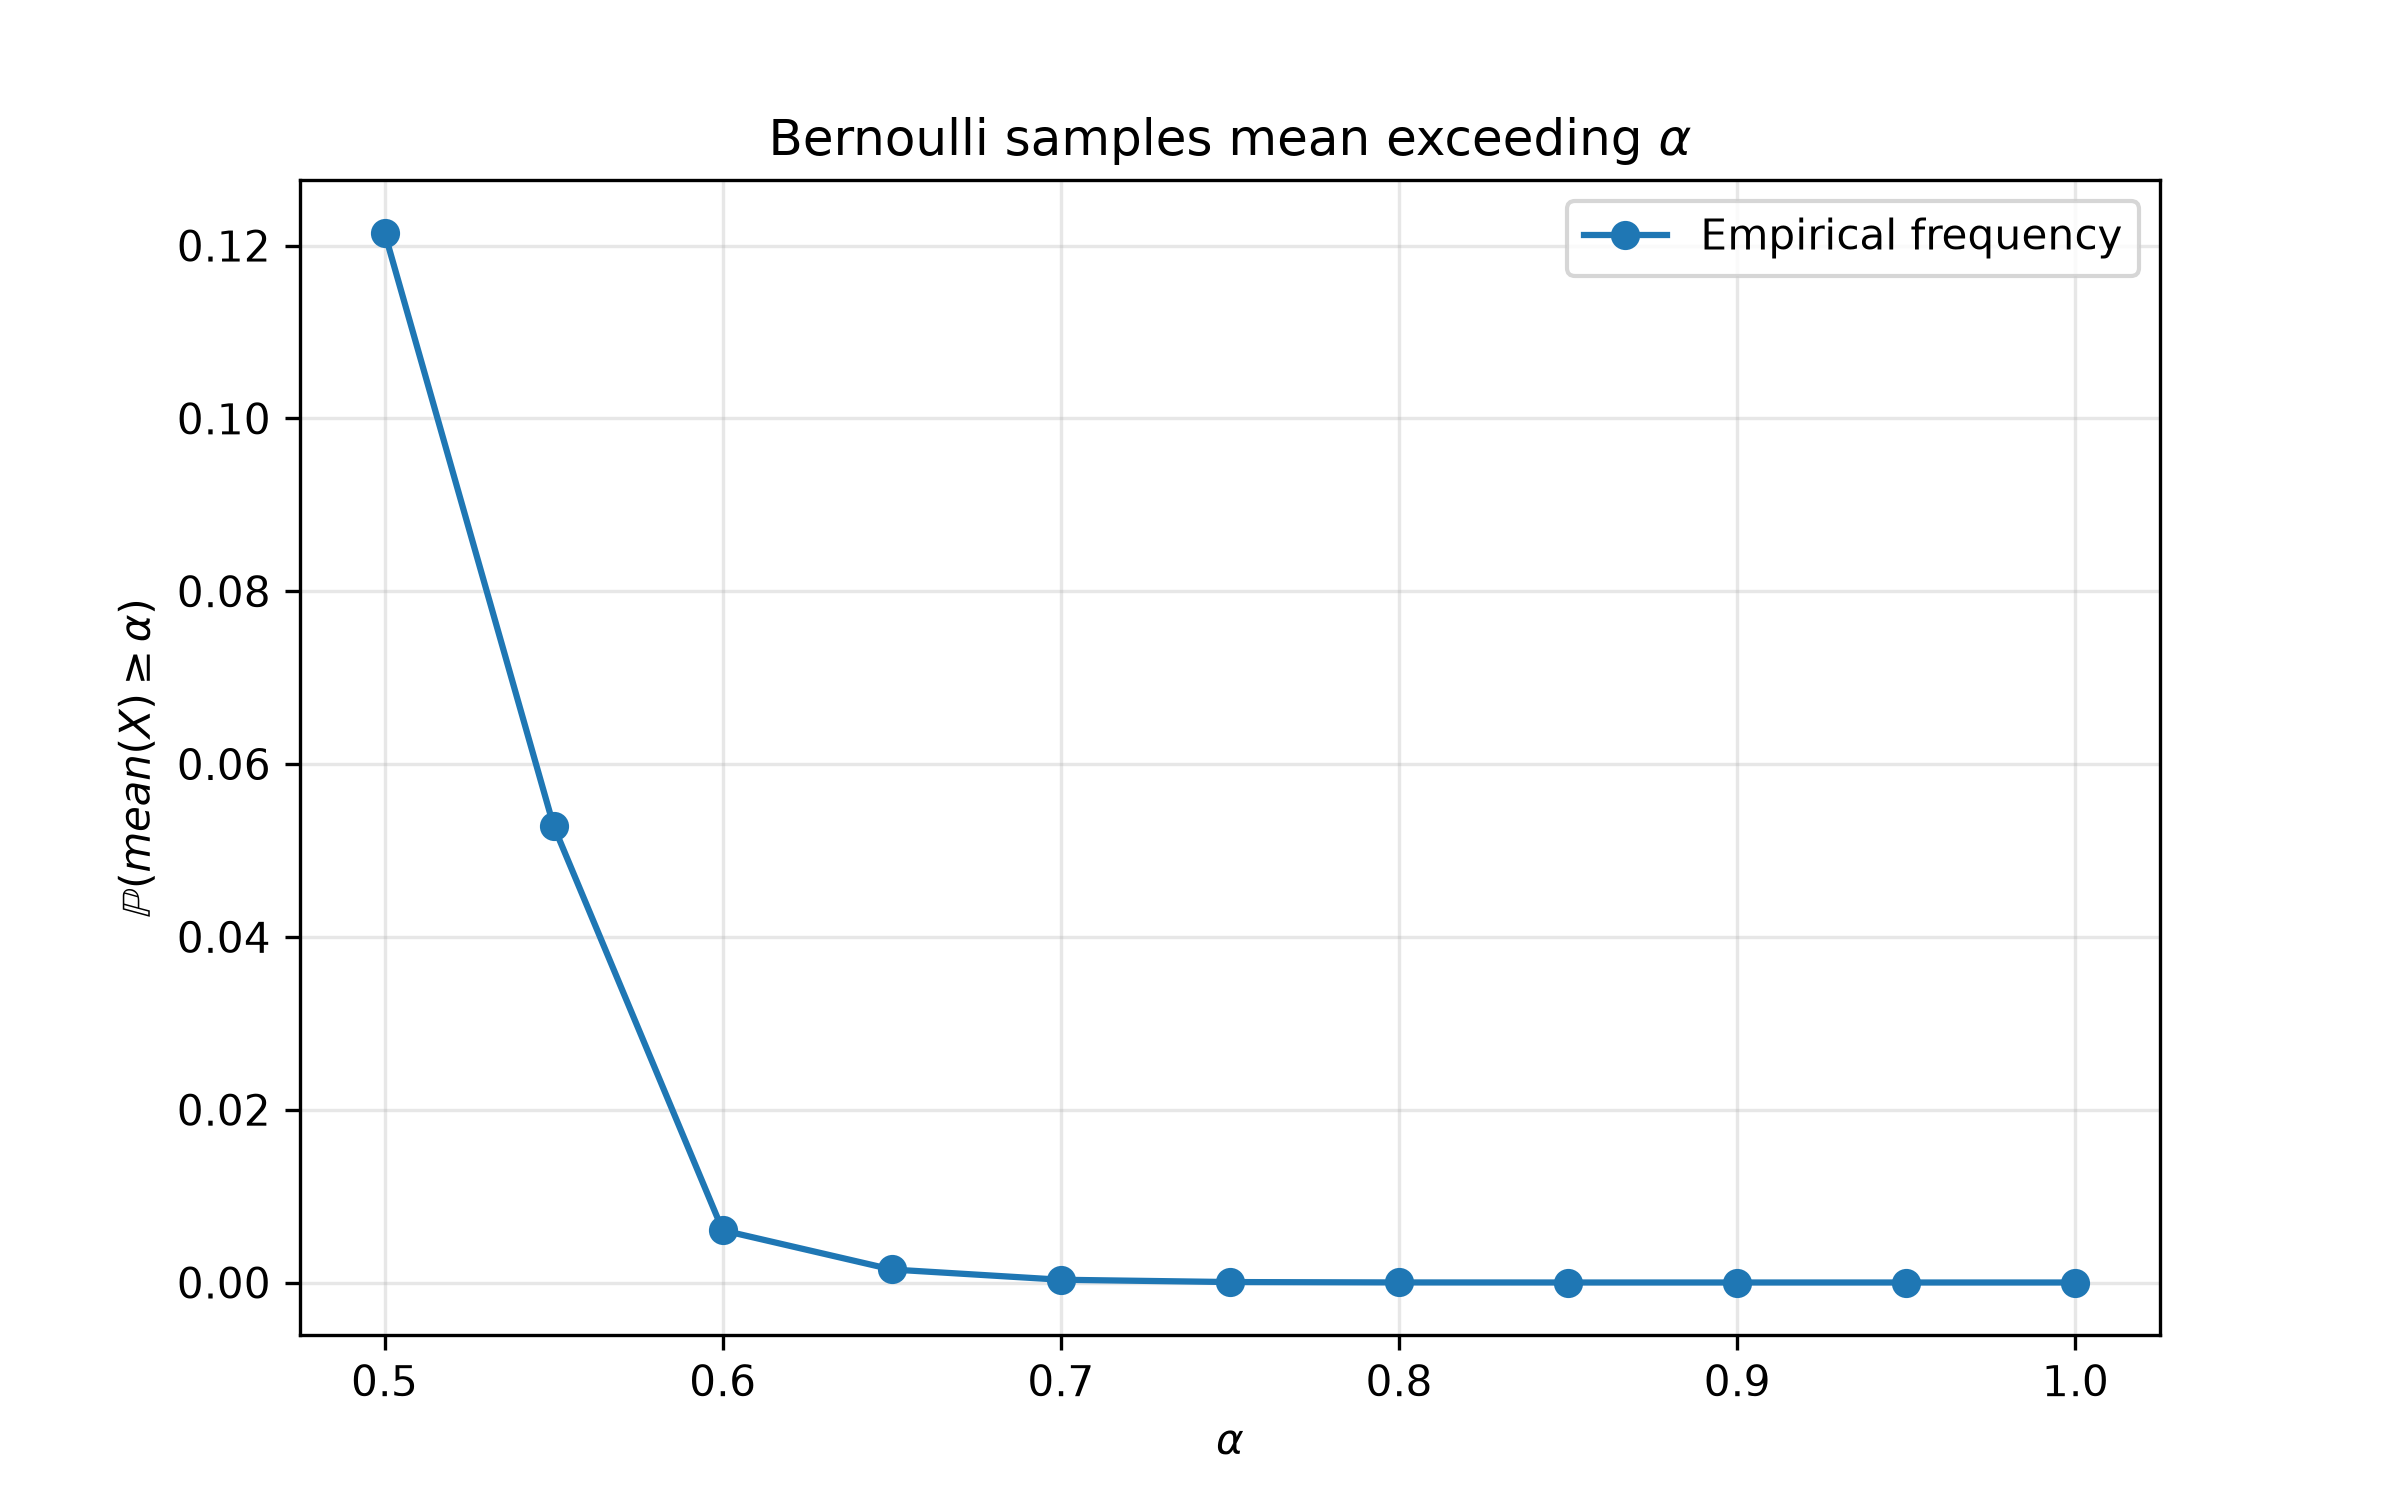
\includegraphics[width=0.75\linewidth]{illustration-of-inequalities/plots/ef.png}
    \caption{Empirical frequency of Bernoulli sample means exceeding $\alpha$}
    \label{fig:ef}
\end{figure}

\paragraph{2.}

Since each $X_i \in \{0,1\}$, the sum $\sum_{i=1}^{20} X_i$ can only result in
$0, 1, \dots, 20$, and the sample mean in $0, 0.05, 0.10, \dots, 1$.
Therefore, taking $\alpha = 0.51$ instead of $\alpha = 0.5$ gives exactly the same
probability as $\alpha = 0.55$.

\newpage

\paragraph{3.}

\begin{lstlisting}
def markov_bound(alphas, expected_value):
    return np.minimum(expected_value / alphas, 1.0)

mean_X = p
markov = markov_bound(alphas, mean_X)
\end{lstlisting}

\begin{figure}[H]
    \centering
    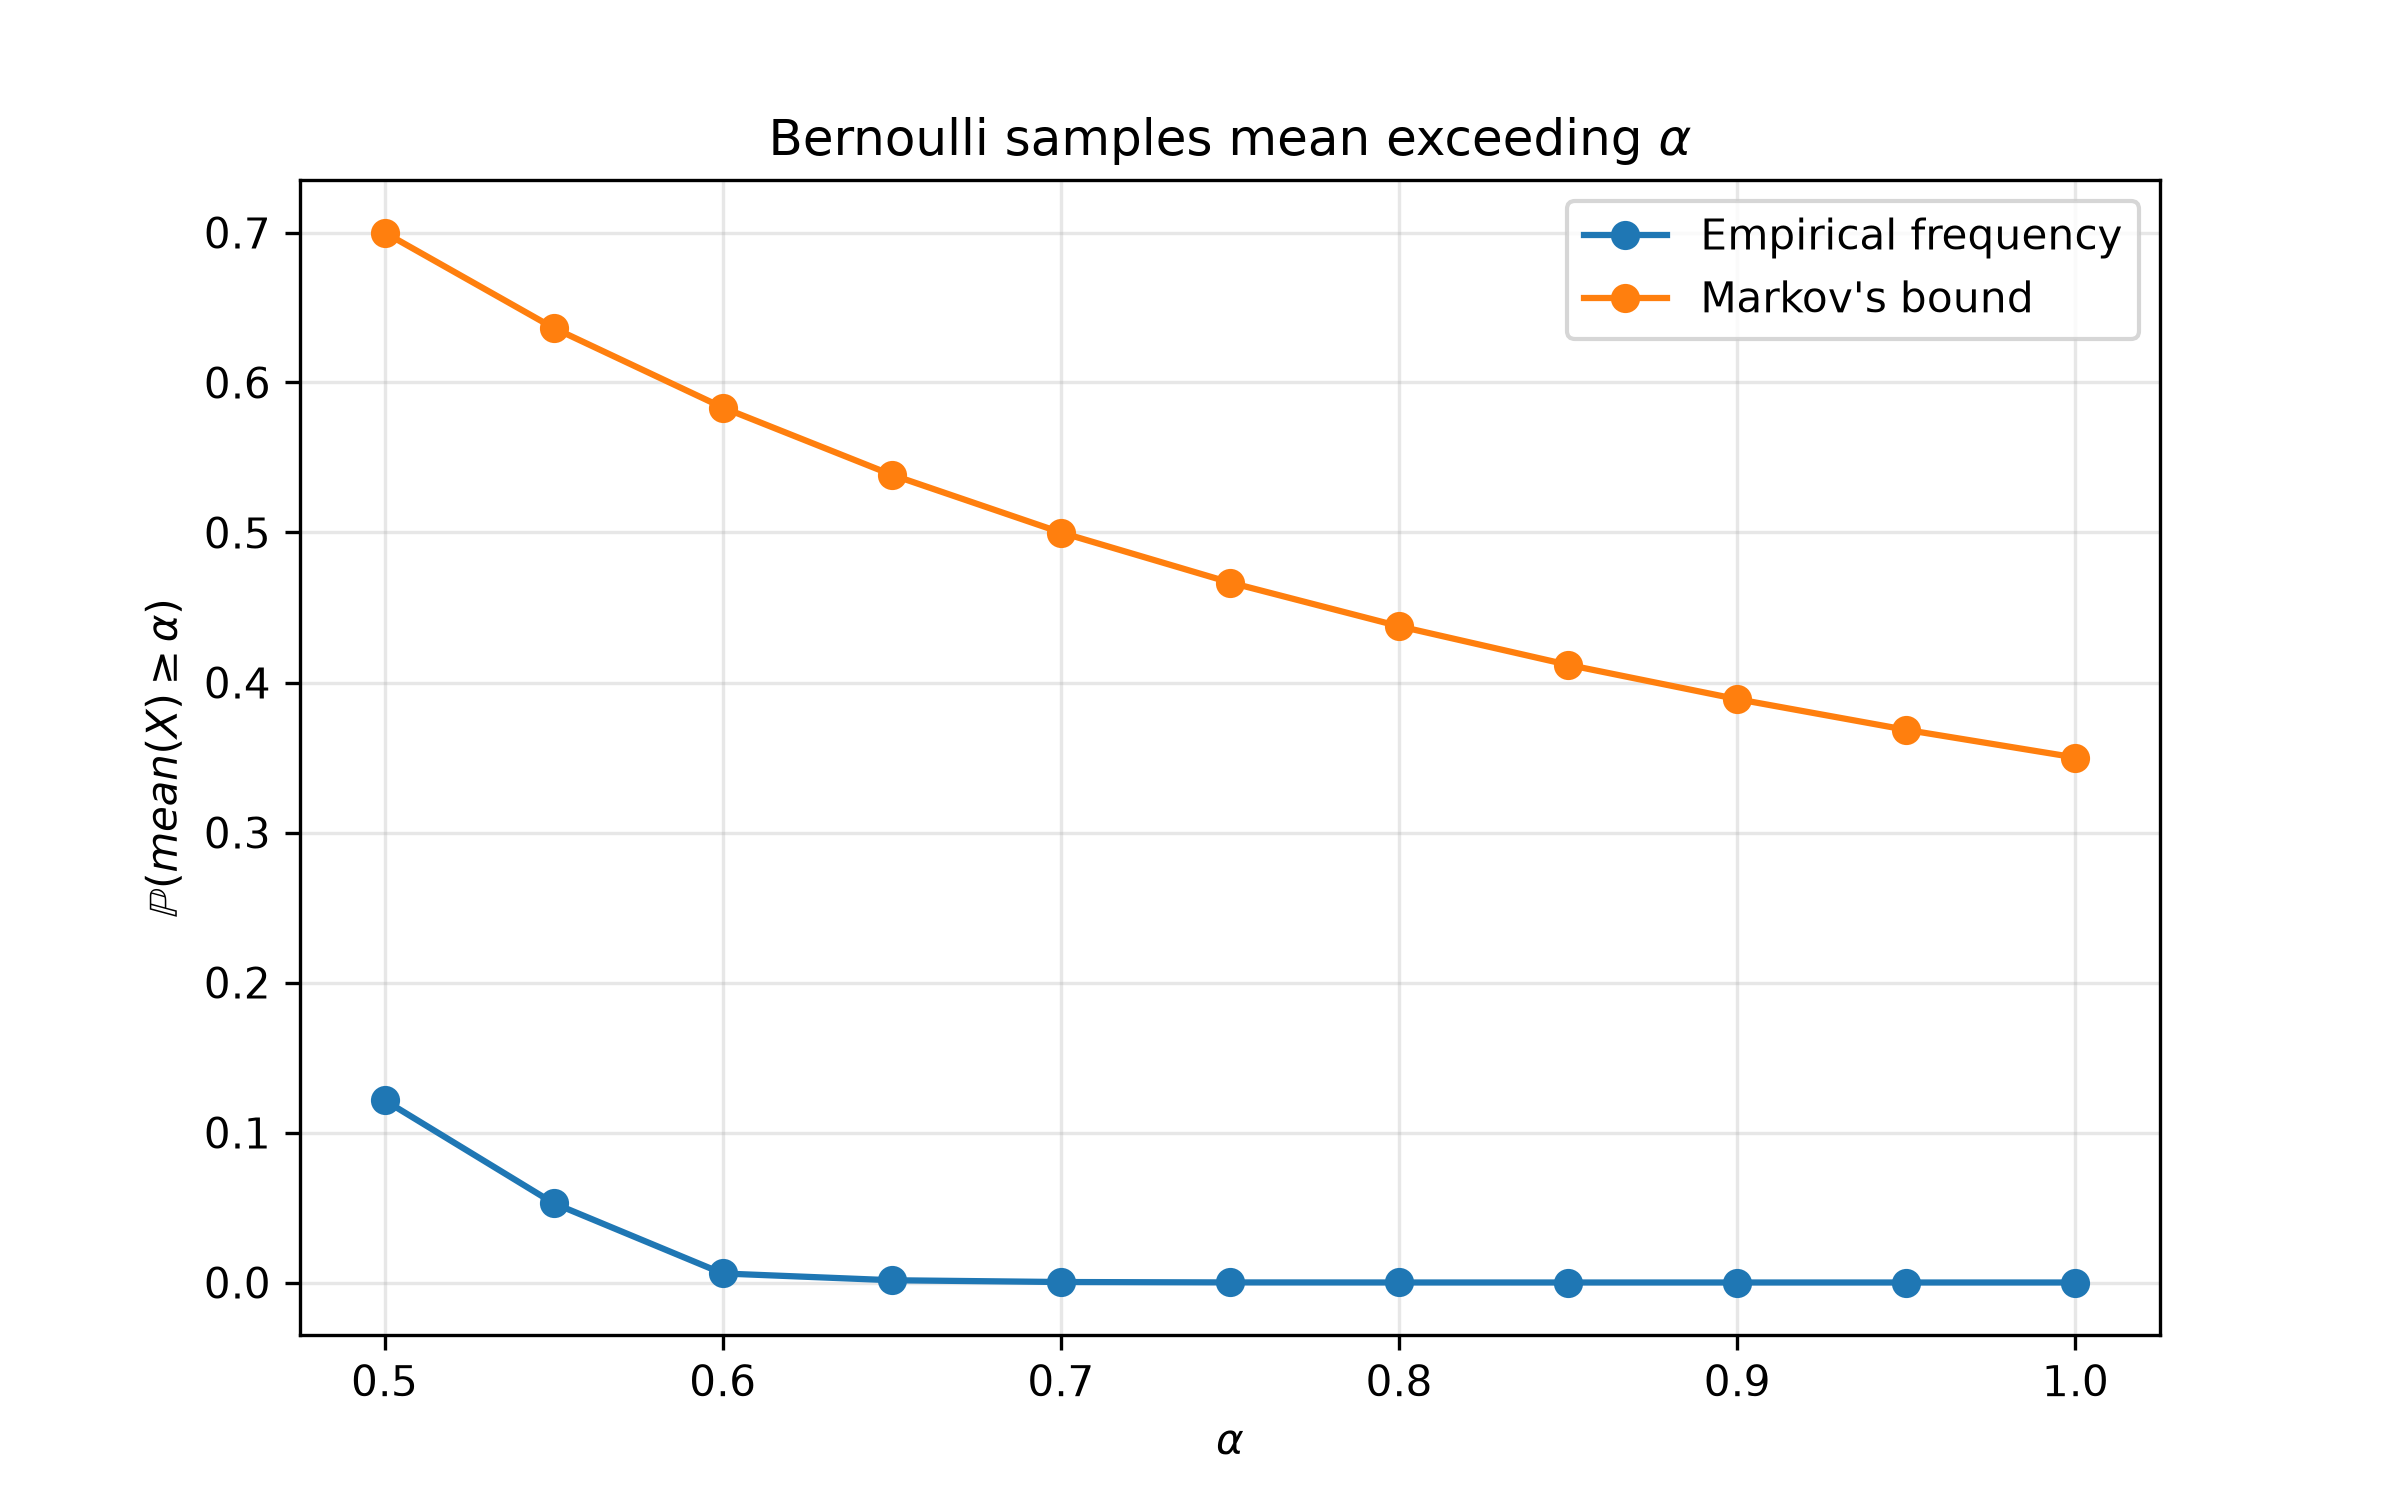
\includegraphics[width=0.75\linewidth]{illustration-of-inequalities/plots/ef_markov.png}
    \caption{Empirical frequency and Markov's bound of Bernoulli sample means exceeding $\alpha$}
    \label{fig:ef_markov}
\end{figure}

\newpage

\paragraph{4.}

\begin{lstlisting}
def chebyshev_bound(alphas, mean, var, n):
    # P(|X - E[X]| >= eps) => we use eps = a - E[X]
    eps = alphas - mean
    bound = np.where(eps > 0, var / (n * np.square(eps)), 1.0)
    return np.minimum(bound, 1.0)

var_X = p * (1 - p)
chebyshev = chebyshev_bound(alphas, mean_X, var_X, n)
\end{lstlisting}

\begin{figure}[H]
    \centering
    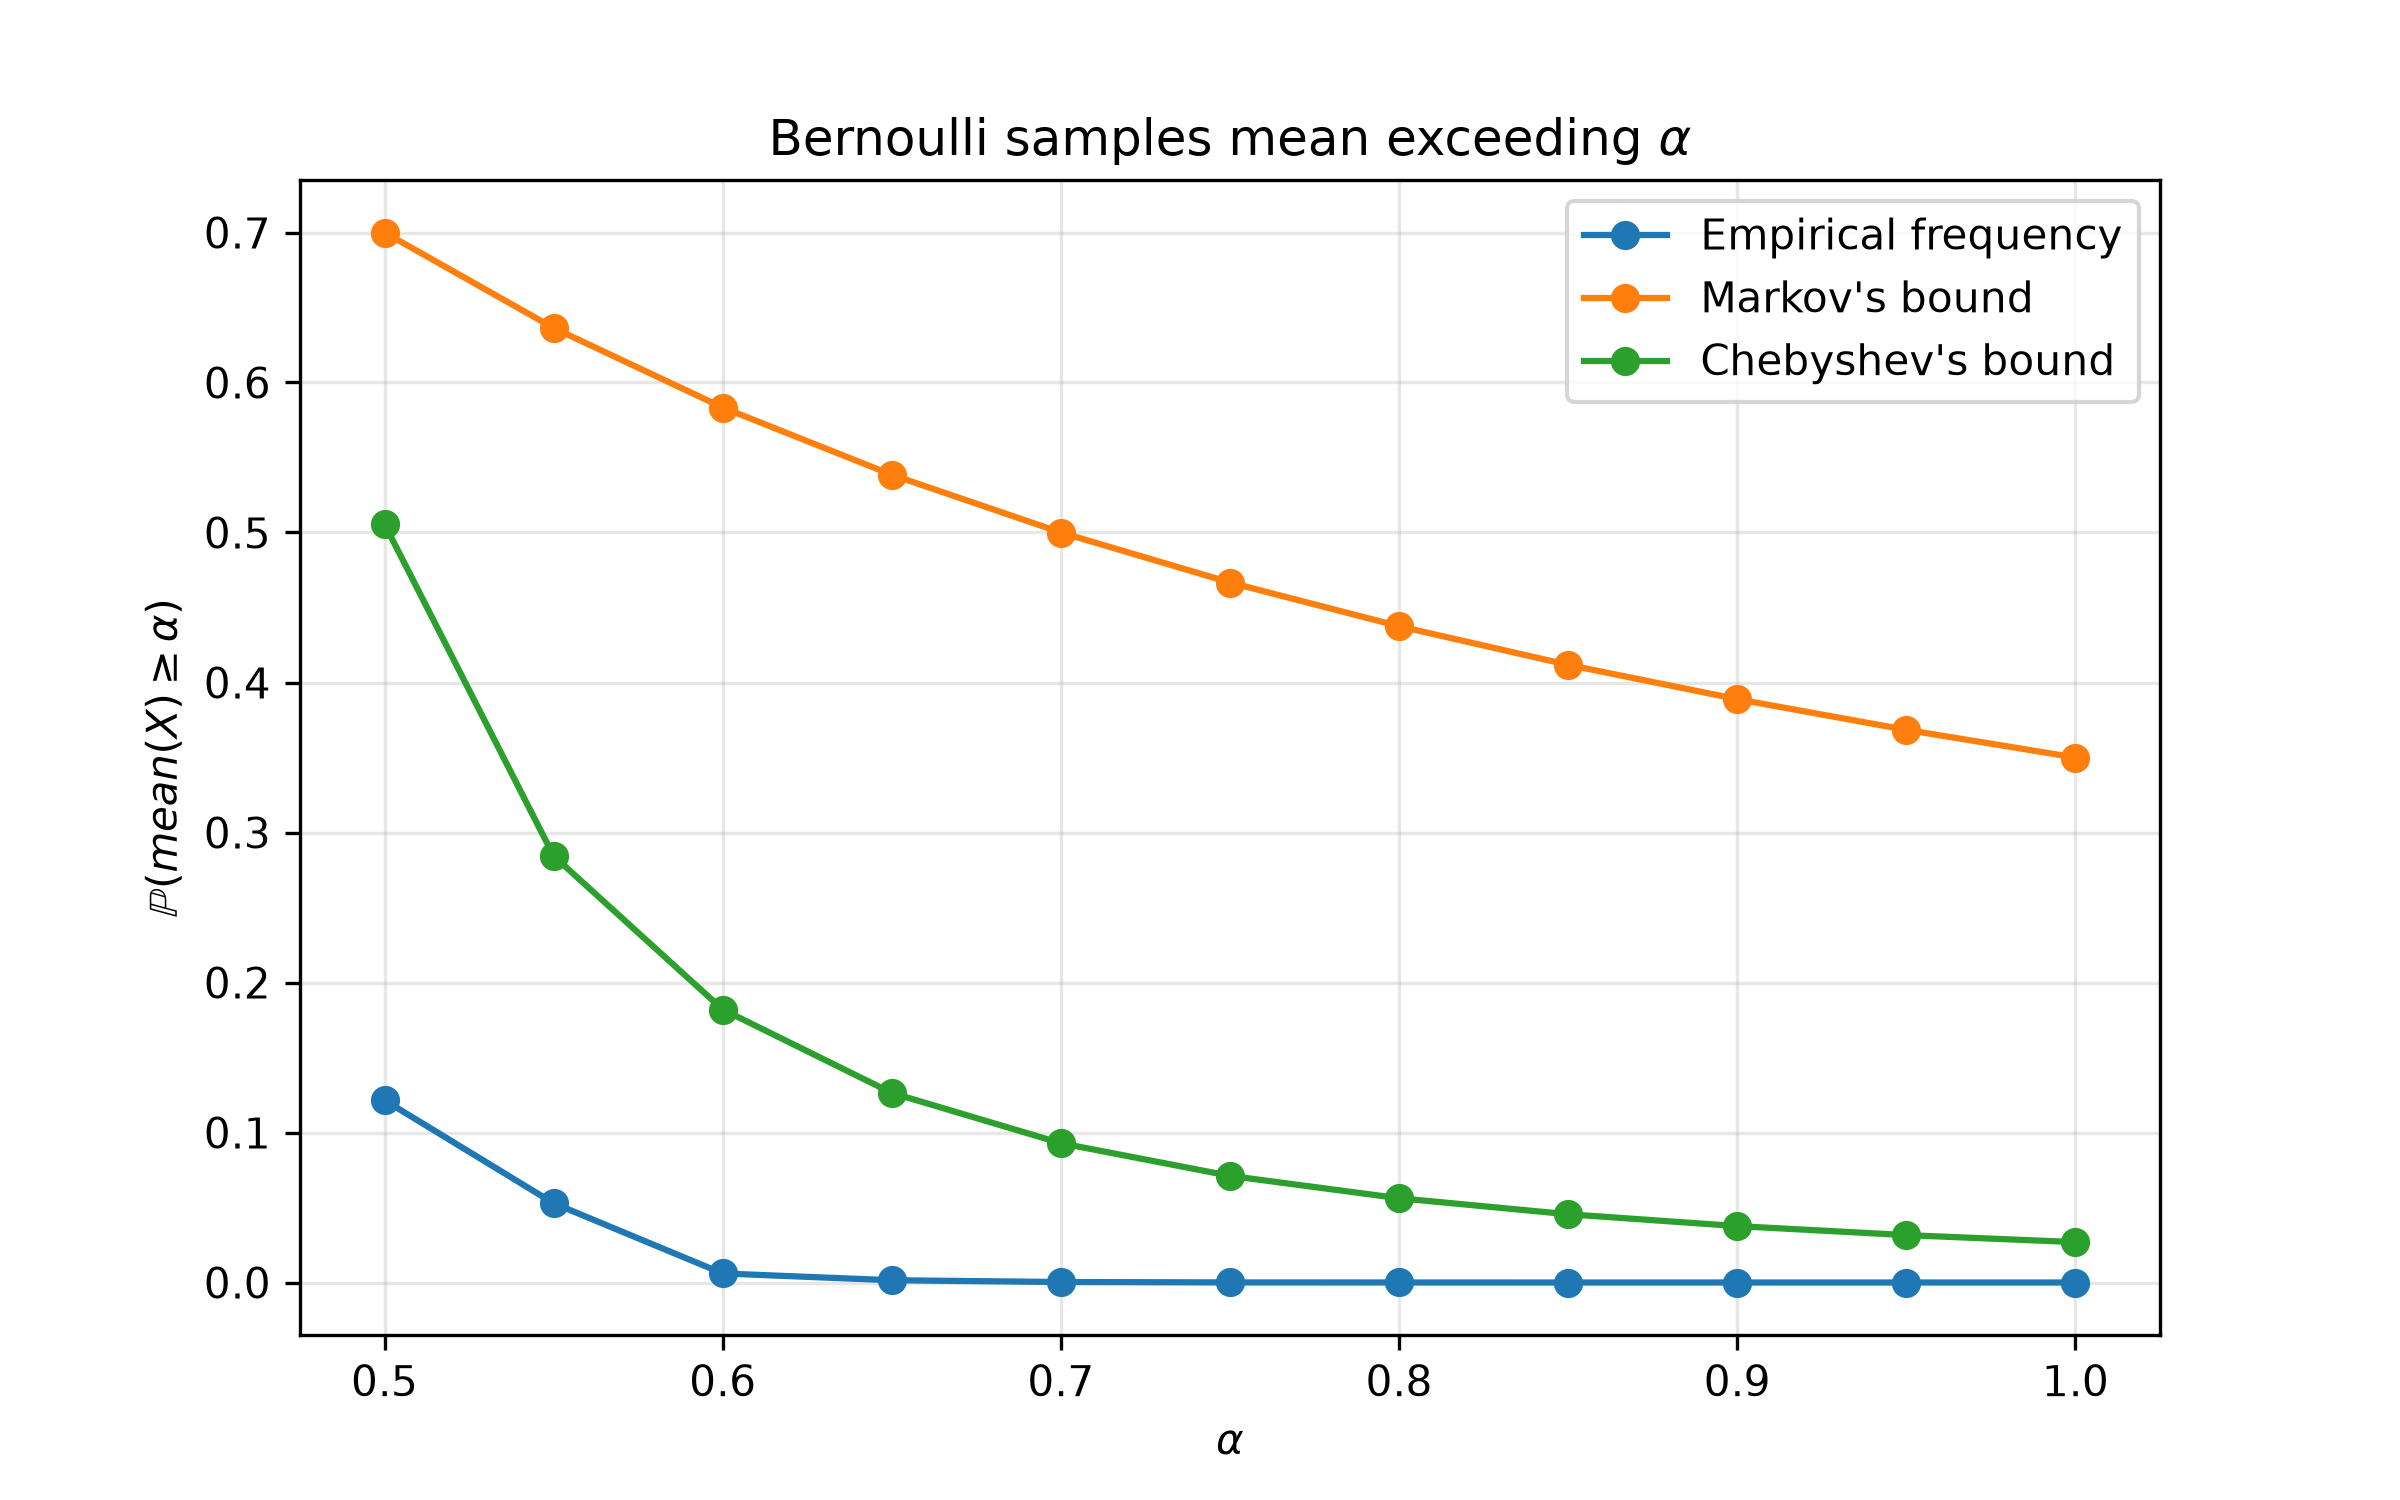
\includegraphics[width=0.75\linewidth]{illustration-of-inequalities/plots/ef_markov_chebyshev.png}
    \caption{Empirical frequency, Markov's bound and Chebyshev's bound of Bernoulli sample means exceeding $\alpha$}
    \label{fig:ef_markov_chebyshev}
\end{figure}

\newpage

\paragraph{5.}

\begin{lstlisting}
def hoeffding_bound(alphas, mean, n):
    eps = alphas - mean
    bound = np.where(eps > 0, np.exp(-2 * n * np.square(eps)), 1.0)
    return np.minimum(bound, 1.0)

hoeffding = hoeffding_bound(alphas, mean_X, n)
\end{lstlisting}

\begin{figure}[H]
    \centering
    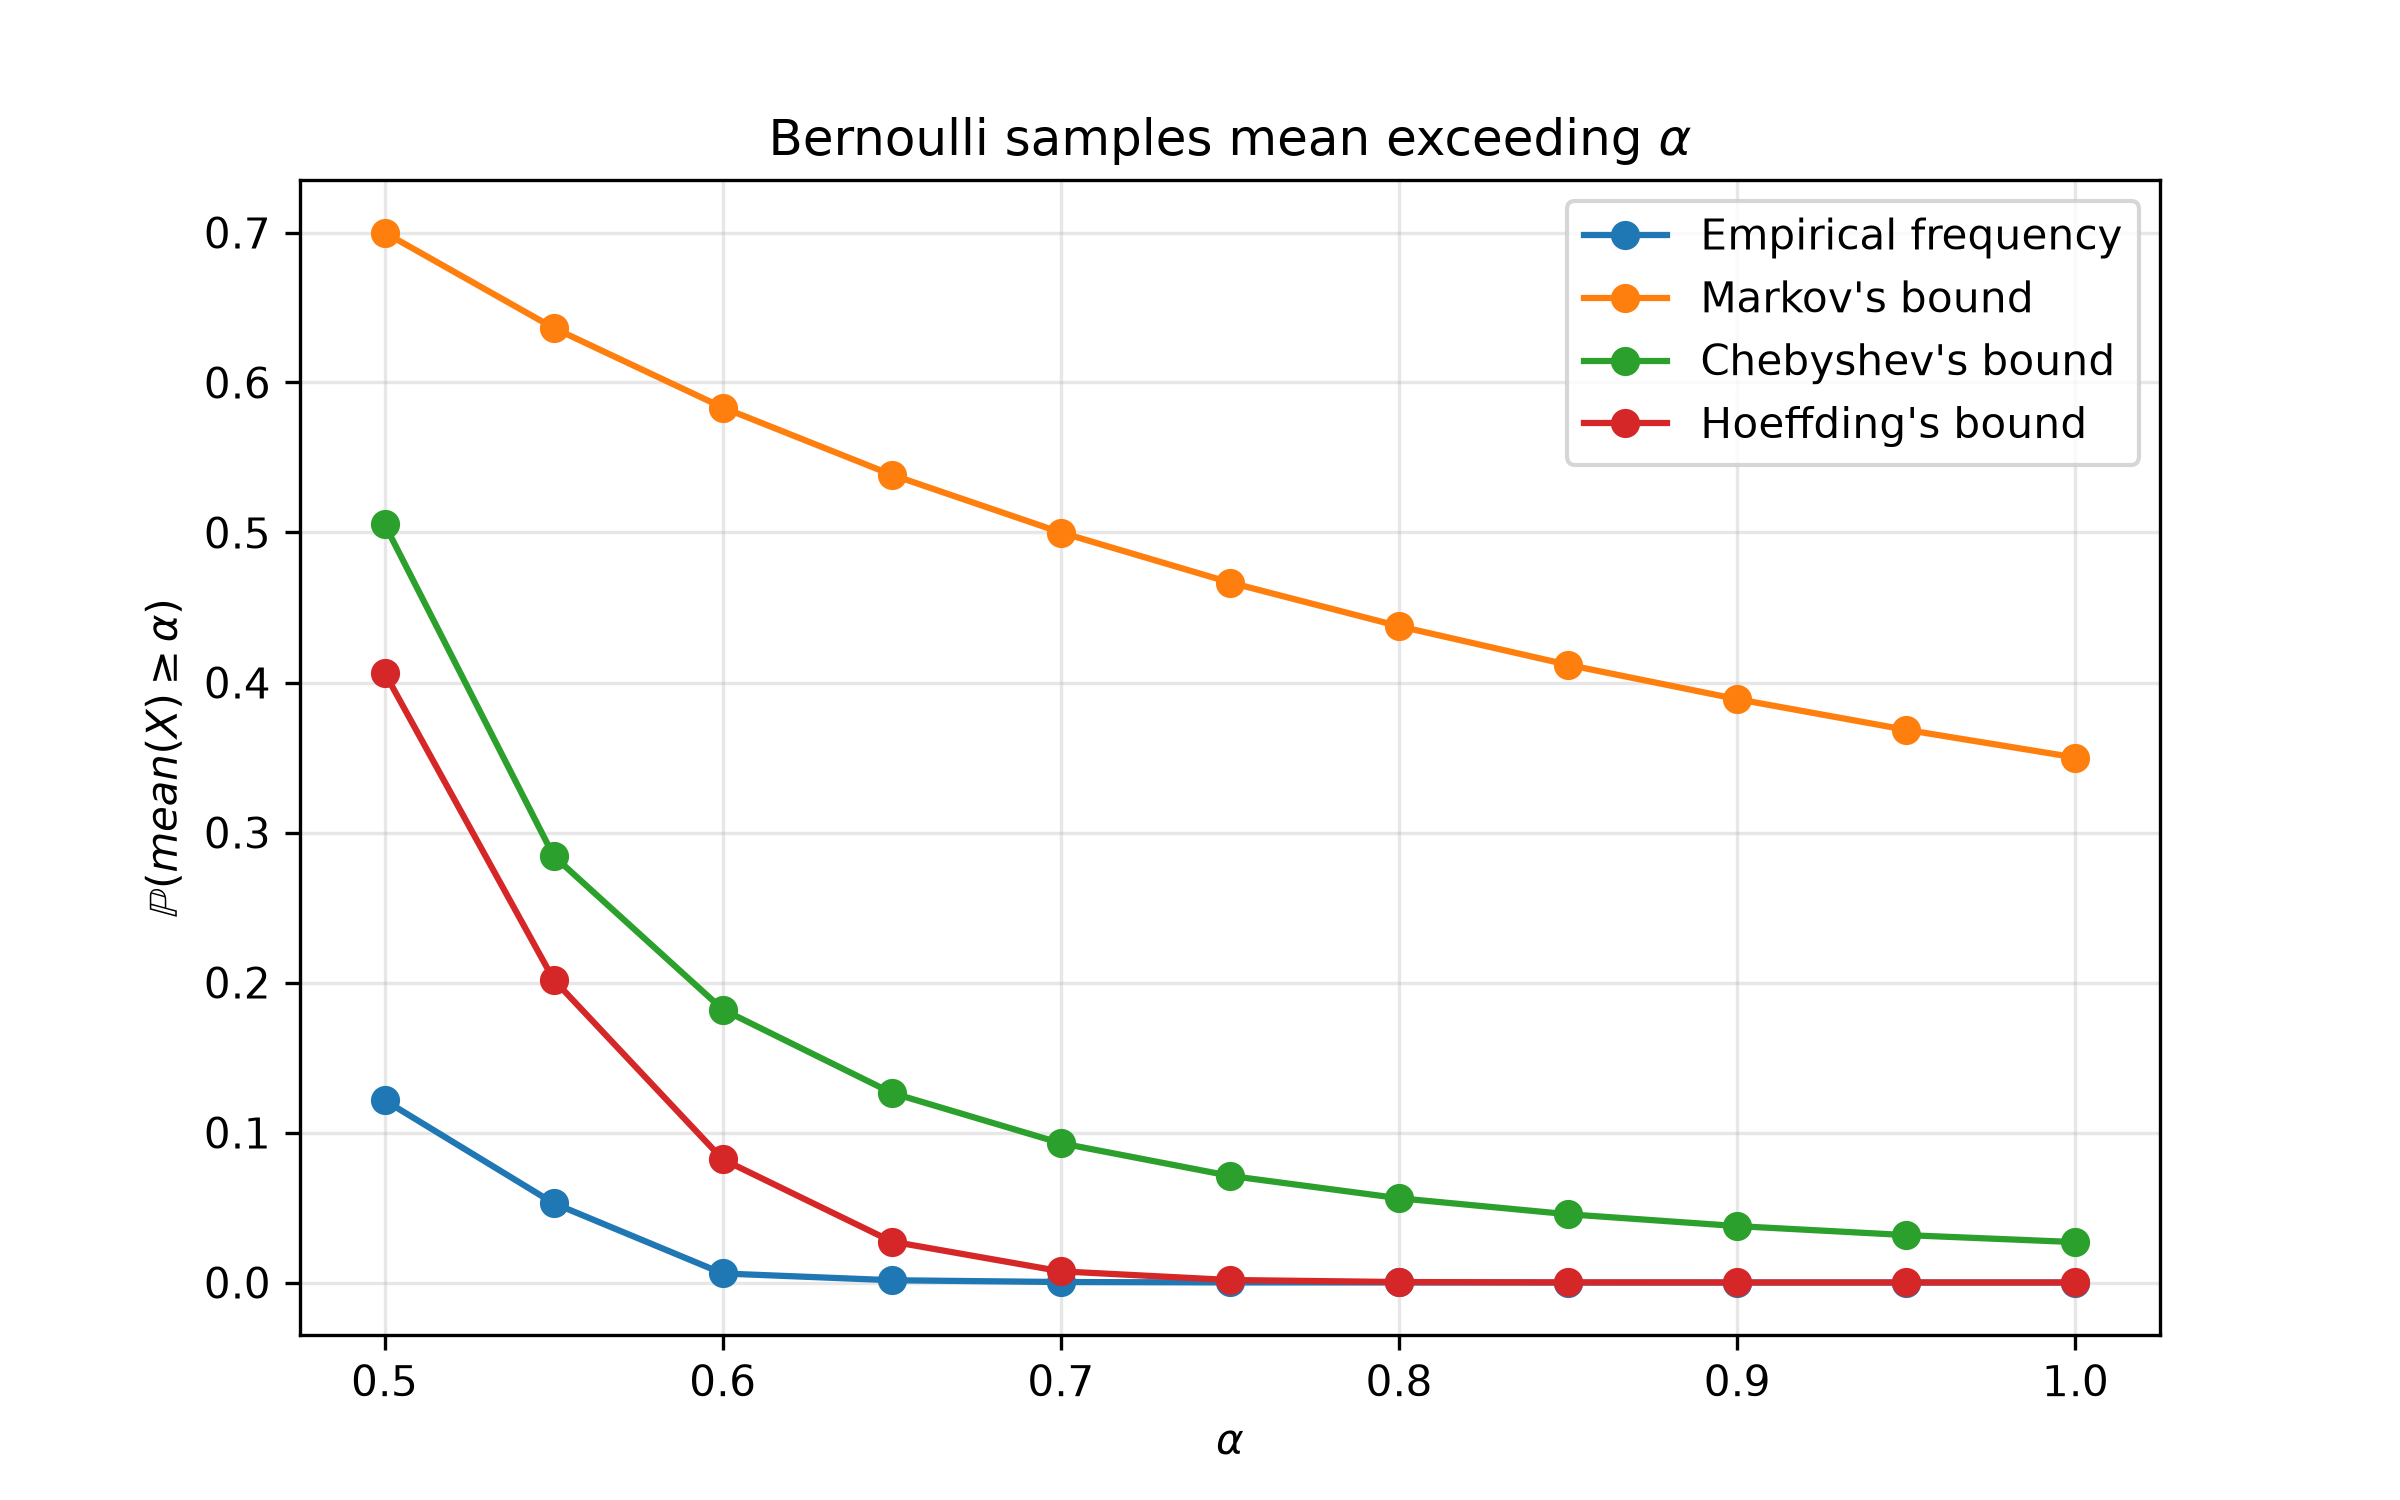
\includegraphics[width=0.75\linewidth]{illustration-of-inequalities/plots/ef_markov_chebyshev_hoeffding.png}
    \caption{Empirical frequency, Markov's bound, Chebyshev's bound and Hoeffding's bound of Bernoulli sample means exceeding $\alpha$}
    \label{fig:ef_markov_chebyshev_hoeffding}
\end{figure}

\paragraph{6.}

The empirical frequency is by far the smallest curve, decaying sharply as
$\alpha$ grows past the mean $p = 0.35$. All three bounds lie above (or
match) the true probability for every $\alpha$, with some differences:

\begin{itemize}
    \item \textbf{Markov's bound} is the loosest by a wide margin, as it only
    decays as $1/\alpha$.
    \item \textbf{Chebyshev's bound} is tighter than Markov's for most of the
    range, since it additionally exploits the variance of the samples, but it
    still decays only polynomially in $\alpha$.
    \item \textbf{Hoeffding's bound} is by far the tightest of the three, because
    it decays exponentially in $n(\alpha - p)^2$.
\end{itemize}

\paragraph{7.}

$$
\begin{aligned}
\sum_{i=1}^{20} X_i \sim \mathrm{Binomial}(20, 0.35) & \implies
\mathbb{P}(\hat{\mu} \ge \alpha) = \mathbb{P}\!\left(\sum_i X_i \ge 20\alpha\right) \\
\mathbb{P}(\hat{\mu} \ge 1) &= \mathbb{P}\!\left(\textstyle\sum_i X_i \ge 20\right) \approx 7.610 \times 10^{-10} \\
\mathbb{P}(\hat{\mu} \ge 0.95) &= \mathbb{P}\!\left(\textstyle\sum_i X_i \ge 19\right) \approx 2.903 \times 10^{-8}
\end{aligned}
$$

\paragraph{3.b [optional, 0 points]}

\end{document}
